\begin{center}
    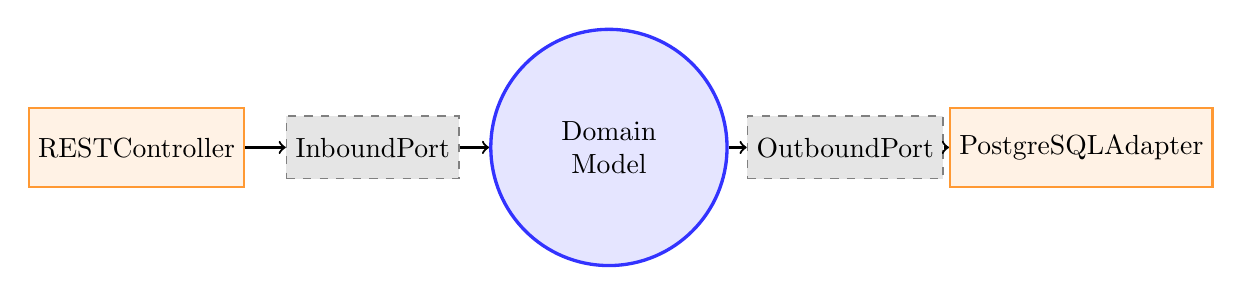
\begin{tikzpicture}[node distance=2cm]
        % Style Definitions
        \tikzstyle{core} = [circle, draw=blue!80, fill=blue!10, very thick, minimum size=3cm, align=center]
        \tikzstyle{adapter} = [rectangle, draw=orange!80, fill=orange!10, thick, minimum size=1cm]
        \tikzstyle{port} = [rectangle, draw=gray, fill=gray!20, dashed, minimum size=0.8cm]
    
        % Nodes
        \node (domain) [core] {Domain \\ Model};
        \node (inport) [port, left of=domain, xshift=-1cm] {Inbound \\ Port};
        \node (outport) [port, right of=domain, xshift=1cm] {Outbound \\ Port};
        \node (web) [adapter, left of=inport, xshift=-1cm] {REST \\ Controller};
        \node (db) [adapter, right of=outport, xshift=1cm] {PostgreSQL \\ Adapter};
    
        % Arrows
        \draw[->, thick] (web) -- (inport);
        \draw[->, thick] (inport) -- (domain);
        \draw[->, thick] (domain) -- (outport);
        \draw[->, thick] (outport) -- (db);
    
    \end{tikzpicture}
    \end{center}